\documentclass[aps,prl,10pt,twocolumn,floatfix]{revtex4-2}
\usepackage{chngpage}
\usepackage{graphicx}
\usepackage{dcolumn}
\newcolumntype{d}{D{.}{.}{-1}}
\usepackage{url}
\usepackage{amsmath}
\usepackage[version=3]{mhchem}
\usepackage{graphicx}
\usepackage{esvect}
\usepackage{circuitikz}
\usepackage{physics}

\bibliographystyle{apsrev4-2}


\begin{document}

\begin{abstract}
%What is the motivation?
%What did you do?
%What were the results?
%Conclusion
\end{abstract}


\title{Lab \#2: Percise Measurement of Gravity Using Kater's Pendulum}
\author{Corbin T. Rochelle (ctr233)}
\date{\today}
\affiliation{Department of Physics and Astronomy\\Mississippi State University\\Mississippi State, MS 39762-5167}
\date{\today}

\maketitle

\section{Introduction}\label{Intro}
% Lead Up to Creation
Prior to the creation of Kater's Pendulum, the best measurement for finding the local value of gravity was using an almost massless thread that was fixed at one end and have a metal sphere connected to the other. 
This method yielded a result to the values of gravity although this method had one major flaw, angular momentum.
When the metal sphere swung from the cord, sometimes the sphere would wobble due to many external factors and cause some of the pendulums energy to be lost to angular momentum \cite{BeforeKater}. 
% Invention
This reason caused captain Henry Kater to devise and create his own pendulum in 1817\cite{KatersWork}!
His new pendulum had two major improvements to the old design, being fixed and being compound. 
% How Does it Work
Instead of having to swing from a cord, the pendulum was solid metal rod, so none of the energy was lost to anguar momentum. 
This alone made the measurement much more precise!
The pendulum was also compound, meaning it has two weights, instead of one, that could offset each other and add more mass to the system to negate air friction and like retardent forces. 
The two wieghts consisted onf one heavy, fixed one at one end and a small, moveable one at the other. 
This allows the one small weight to be adjusted, either on a macro or micro scale, to influence the center of mass of the pendulum.  

\section{Theory}\label{Theory}
% Derivation of Formula 
We know from the lab manual that ``if the period of oscillation of a physical pendulum about one axis a distance $l_1$ from the center of mass (i.e., the radius of gyration) is $T_1$ while the period of oscillation about the other pivot a distance $l_2$ from the center of mass is $T_2$, then the acceleration due to gravity is given by\cite{Manual}"
\begin{equation}\label{EQ1}
\frac{8\pi^2}{g}=\frac{T_1^2+T_2^2}{L}+\frac{T_1^2-T_2^2}{l_1-l_2}
\end{equation}
where $g$ is the local gravity, $T_1$ is the upright period measure, $T_2$ is the upside-down period measure, $L$ is the length of the rod, $l_1$ is the length to the adjustable weight from the top knife-edge, and $l_2$ is the length from the adjustable weight to the bottom knife-edge. 
This is true of all physical pendulums, although it requires the measurement of four different quantities to determine $g$. 
If we adjust the small, moveable weight to make the periods, $T_1$ and $T_2$, equal each other, we can cancel one of the fractions and drop the number of values we must measure to 3!
The periods being equal makes equation \ref{EQ1} become
\begin{equation}\label{EQ2}
\frac{8\pi^2}{g}=\frac{2T^2}{L}+0
\end{equation}
where $T=T_1=T_2$.
We can now rearrange equation \ref{EQ2} to solve for $g$:
\begin{equation}
g=\frac{4\pi^2L}{T^2}
\end{equation}

\section{Experiment}
% What did you do?

\section{Data Analysis}
% Explain the Results 
\begin{figure}\label{1stGraph}
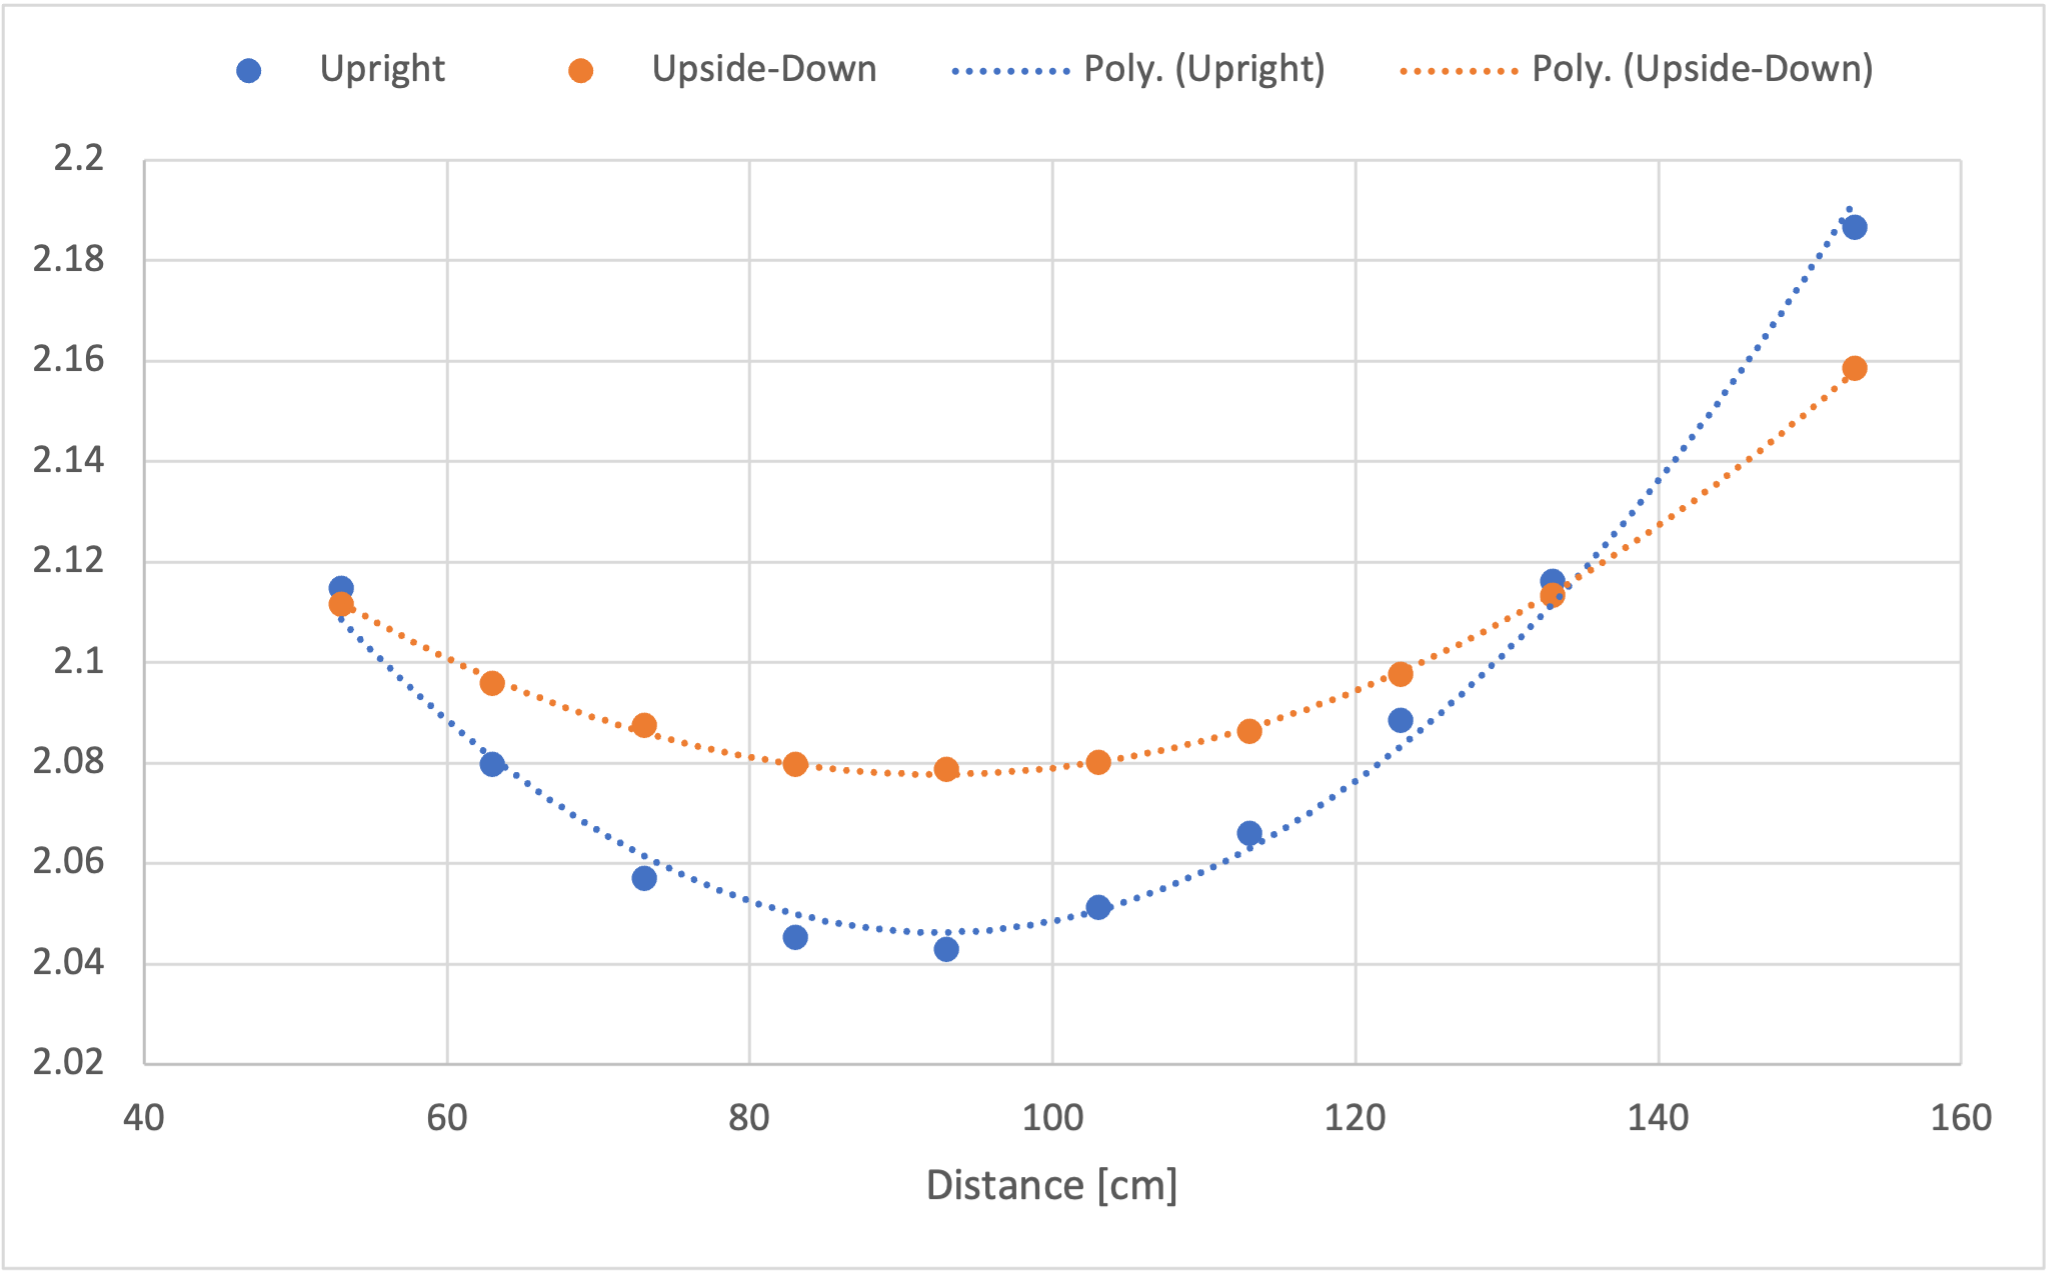
\includegraphics[width=230px]{FirstMeasurement.png}
\caption{The Graph of Large Movements in the Small Weight}
\end{figure}

For the first measurement, to obtain the rough estimate of where $T_1=T_2$ was located, we obtained Figure \ref{1stGraph}. 

\section{Conclusion}
% Conclusion 


\begin{thebibliography}{9}
\bibcite{BeforeKater} Britannica, T. Editors of Encyclopaedia. \textit{pendulum} (Encyclopedia Britannica, September 1, 2021). \url{https://www.britannica.com/technology/pendulum}.
\bibcite{KatersWork} H. ~Kater, \textit{An Account of Experiments for determining the Length of the Pendulum Vibrating Seconds}, (The Latitude of London, 1817).
\bibcite{Manual} J. ~Winger, \textit{Percise Measurement of g Using Kater’s Pendulum}, (Mississippi State University).
\end{thebibliography}

\end{document}
